\section{Introduction}
\label{sec:introduction}

Embodied artificial intelligence (AI) is extending autonomous machines from structured, instrumented spaces into physical environments with uncertain contacts, limited visibility, and unreliable external positioning~\cite{liu2025embodied-survey}. A robot must maintain an estimate of its pose, velocity, and internal state while it perceives the environment, plans motion, and applies control. Deep-space vehicles, subterranean platforms, legged robots~\cite{he2024legged-state,ou2024leg-kilo}, and autonomous vehicles use different sensors and motion models, yet their local state-estimation loops repeatedly propagate inertial information and correct it with intermittent observations through recursive Bayesian estimation. The quality and timeliness of this loop determine how reliably the rest of the perception--action system can operate.

This requirement is especially visible in embodied-AI systems~\cite{embodied-ai-survey}. Humanoids and quadrupeds combine inertial, kinematic, contact, and visual measurements at high update rates; a local extended Kalman filter (EKF) or error-state filter often provides the high-rate inertial-propagation and measurement-correction layer even when a separate mapping system supplies global consistency. Consistent fusion of leg kinematics and inertial measurements has been demonstrated for legged robots~\cite{bloesch2012}, while the DARPA Subterranean Challenge shows how localization, mapping, and navigation must remain tightly coupled when robots operate in underground environments~\cite{cerberus2022}. Such robots increasingly depend on large simulation campaigns that vary contact conditions, sensor noise, terrain, and control parameters. GPU-native simulators such as Isaac Gym execute thousands of robot environments concurrently~\cite{isaacgym2021}, so every repeated state-estimation loop in the pipeline must sustain higher throughput.

Downhole traction robots provide a concrete and demanding instance of this broader embodied-autonomy problem. These robots actively convey coiled tubing, toolstrings, and attached tools through highly deviated and horizontal wells, where gravity, friction, and long constrained passages make passive delivery unreliable. Recent field deployments have demonstrated their use in horizontal-well intervention, logging, perforation, and zonal-isolation operations~\cite{he2020downhole-tractor,chawla2024tractor-glide}. As illustrated in \Cref{fig:downhole-tractor}, a surface unit deploys the toolstring through the wellbore while the tractor provides active conveyance along the horizontal section. In the cased horizontal well considered in this study, high temperature and pressure, corrosion, deposits, local deformation, and obstructions can perturb wheel--wall contact and induce slip or short-lived odometry disturbances. Reliable operation therefore requires continuous fusion of inertial and traction measurements through a strapdown inertial navigation system (SINS) supporting an error-state extended Kalman filter, to estimate the robot state and suppress accumulated drift. Before deployment, large simulation campaigns are needed to evaluate sensor noise, slip events, obstacle-induced disturbances, and filter parameters over long trajectories, making downhole traction robot positioning not only a state-estimation problem but also a computationally intensive simulation workload.

\begin{figure}[!t]
  \centering
  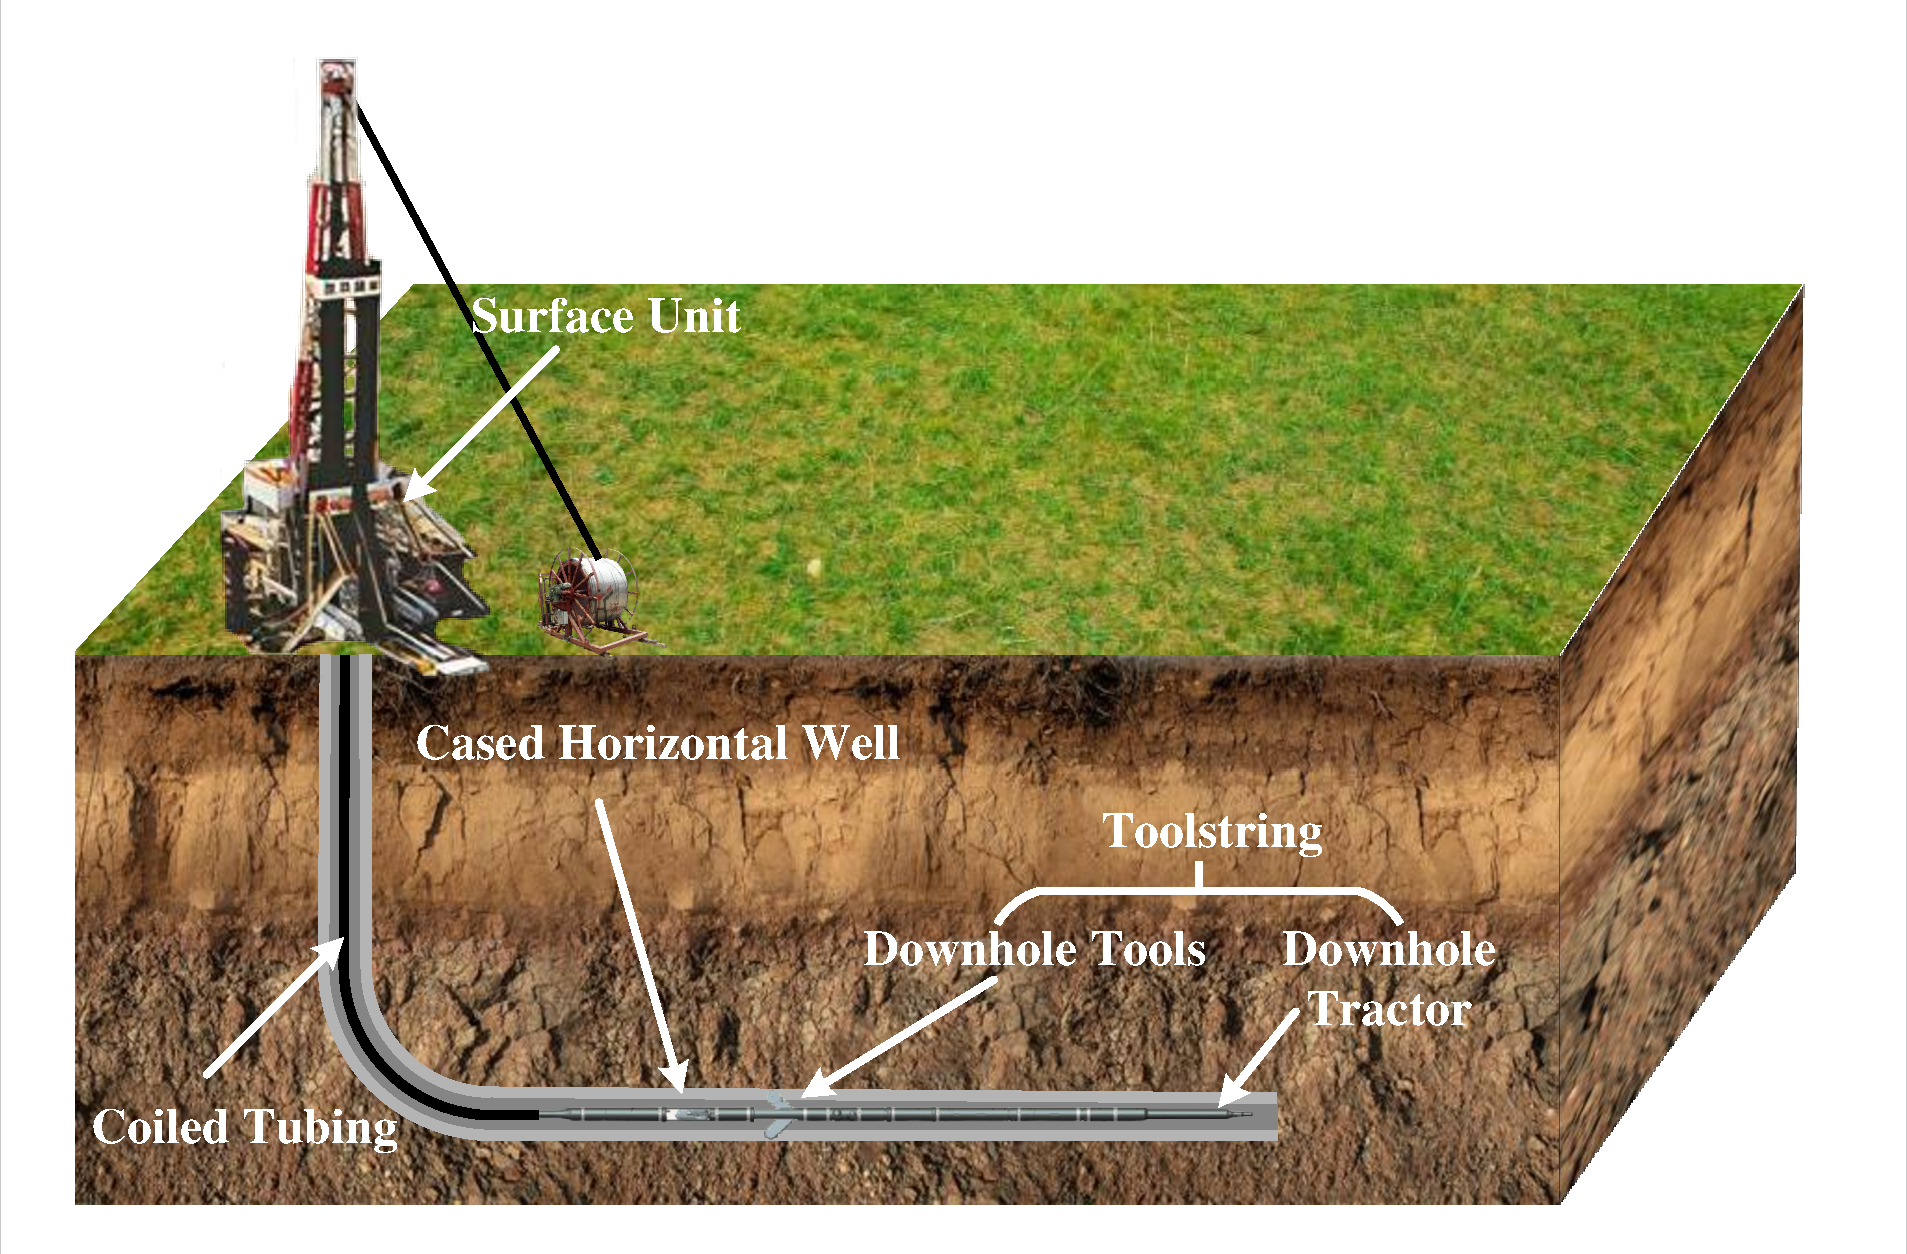
\includegraphics[width=\linewidth]{figures/1-intro-robot.pdf}
  \caption{Schematic of a downhole traction robot conveying a toolstring into the horizontal section of an oil or gas well.}
  \label{fig:downhole-tractor}
\end{figure}

The resulting estimator has an execution pattern that differs from the large, throughput-oriented matrix workloads commonly used to showcase GPUs. Although the simulation campaigns described above are throughput-hungry, each estimator update is a small numerical operation embedded in a long dependency chain, and a direct tensor implementation fragments the computation into many fine-grained device operations. Repeated launches, synchronization, and movement of recurrent state can dominate arithmetic, leaving much of the accelerator underutilized and causing a straightforward GPU port to underperform a CPU implementation. These characteristics motivate an implementation study centered on launch overhead, on-chip state locality, numerical precision, and independent trajectories available at the simulation level.

We develop \textsc{Trident}, a GPU acceleration framework for this workload. It composes three complementary optimizations---operator fusion, component-aware mixed precision, and multi-trajectory batching---which target the dispatch, numerical, and device-occupancy bottlenecks above. The main contributions are as follows:

\begin{itemize}
  \item We diagnose the execution behavior of SINS/EKF simulation and develop a progressive fusion path culminating in a single fused whole-scan Triton kernel that keeps the recurrent filter state on chip and executes a complete trajectory with minimal device dispatch.
  \item We establish a component-aware precision strategy for recursive filtering and evaluate the performance and long-horizon accuracy of fp64 and fp32 recursive arithmetic, fp16 and bfloat16 sensor input, and IEEE versus TensorFloat-32 dot products, including failure cases caused by error accumulation.
  \item We map independent trajectories to CUDA blocks and derive a scaling model that relates batch throughput to accelerator occupancy and register pressure, enabling high-throughput Monte Carlo and parameter-sweep simulation.
\end{itemize}

The remaining sections of this paper are organized as follows. \Cref{sec:background} introduces the positioning model and its computational structure. \Cref{sec:motivation} presents the profiling evidence and optimization requirements. \Cref{sec:methodology} describes the \textsc{Trident} framework. \Cref{sec:evaluation} evaluates performance, accuracy, and scalability. \Cref{sec:related-work} discusses related work and \Cref{sec:conclusion} concludes the paper.
